% Use the University of Michigan thesis class.
% options include report, thesis, debug, backref
\documentclass[thesis]{thesis-gwu}[2016/09/24]

\usepackage{lipsum}

% --------- FRONT MATTER PAGES ---------------------
% Title of the thesis
\title{Solving Nonlinear Equations of One Variable}

% Author name
\author{Shankar Kulumani}

% Previous degrees
\bsdepartment{Astronautical Engineering}
\bsschool{U.S. Air Force Academy}
\bsgrad{May 2009}

\msdepartment{Aeronautics and Astronautics}
\msschool{Purdue University}
\msgrad{December 2013}

% PhD degree commands
% Committee
\showcommitteepage
%\hidecommitteepage
\committee{ %
Taeyoung Lee, Associate Professor of Engineering and Applied Science,\\ 
Dissertation Director\\
Full Name, Title, \\
Dissertation Director/Co-Director/Committee Member
}

% Chair must be entered separately for formatting reasons.
\chair{Taeyoung Lee}
\chairtitle{Associate Professor of Mechanical and Aerospace Engineering}
% Department
\department{Mechanical and Aerospace Engineering}

\phdgrad{May 28, 2015}
\defensedate{May 28, 2015}
% Year of completion for copyright page and perhaps other places
\year=2015 

% Frontispiece
% delete to not print

% Copyright page
%\copyrightholder{Someone else}

% Dedication
\dedication[8]{ %
\textit{to Christine}
}

% Acknowledgments
\acknowledgments{
Lorem ipsum dolor sit amet, consectetur adipiscing elit. 
Integer sagittis, sem nec molestie blandit, dui orci fermentum ex, eu vehicula sapien ipsum consectetur lacus. 
Vivamus non leo ut sem iaculis hendrerit. Duis sed quam ligula. 
Duis fermentum fringilla ante. Etiam scelerisque mi sapien, ac dictum arcu accumsan et. 
Fusce vel purus lacinia, rhoncus sapien id, lobortis libero. 
Vivamus nec odio et felis aliquam eleifend. 
Class aptent taciti sociosqu ad litora torquent per conubia nostra, per inceptos himenaeos. 
Curabitur suscipit ex eget purus fermentum, in facilisis mauris viverra. 
In tincidunt sollicitudin diam, sed volutpat ex vestibulum eget. 
Curabitur maximus porttitor auctor. Sed imperdiet suscipit leo sed congue. 
Aliquam porttitor egestas aliquet. Donec imperdiet blandit odio, eu mollis ex bibendum semper. 
Donec suscipit nisi nisi, nec tempor dolor eleifend a. 
Aliquam rutrum lacus eget tellus suscipit, et ullamcorper elit eleifend.
}

% Preface
\preface{Ut ornare ut risus in condimentum. 
Proin vitae est sit amet eros hendrerit efficitur. 
Pellentesque ultricies turpis a euismod malesuada. 
Nam ut ante sollicitudin, blandit erat vel, dignissim purus. 
Cras molestie luctus dolor non dapibus. Donec ac hendrerit nulla. 
Vivamus faucibus velit at imperdiet posuere. 
Suspendisse pharetra sit amet purus id dictum.

}

\prologue{
Fusce imperdiet lectus vitae sapien sollicitudin, ac mollis nulla feugiat. 
Mauris vitae tellus non elit faucibus volutpat. 
Phasellus congue, urna a luctus dictum, ligula urna commodo ante, at dignissim nunc nulla et ligula. 
Cras tincidunt, diam et imperdiet vulputate, felis erat malesuada nibh, quis porttitor turpis libero at ligula. 
Etiam ut lacus euismod, interdum erat eget, lobortis neque. 
Suspendisse maximus sem in tempor facilisis. Aenean sed quam enim. 
Mauris posuere libero magna, non posuere nisi luctus vel. 
Vestibulum porttitor varius nisi, at volutpat ipsum hendrerit nec. 
In sit amet risus congue, sodales erat in, venenatis tortor. 
Ut semper placerat nunc, nec laoreet orci egestas aliquet. 
Phasellus commodo vel mauris eu maximus. 
Morbi id vulputate nisl.
}

\foreword[2]{
Fusce in eros a diam molestie fermentum. 
In nisl neque, egestas at sem at, ornare cursus eros. 
Aenean euismod erat pretium, sollicitudin leo quis, vestibulum mauris. 
Proin commodo pharetra aliquam. Aliquam in purus tortor. 
Nulla viverra neque ac justo fringilla facilisis. 
Suspendisse et pellentesque sem. 
Integer laoreet nibh enim, at sollicitudin lectus sodales at. 
Mauris at vestibulum ex. Sed in sapien in ante sollicitudin ultrices. 
Pellentesque tincidunt est ut massa vehicula, ac lacinia justo vehicula. 
Quisque imperdiet feugiat justo a vulputate. Sed non consequat purus, eu pellentesque risus. 
Phasellus leo felis, eleifend et tincidunt et, commodo non enim.
}

% commands to show or hide front matter pages

\showcopyright
\showabstract
\showcommitteepage
\showdedication
\showacknowledgments
\showpreface
\showprologue
\showforeword
% ------------ TABLE OF CONTENTS ----------------------
% Commands to hide or show lists of figures, tables, etc.
\showlistoffigures
\showlistoftables
\hidenomenclature

% Definition of any abbreviations used.
\abbreviations{
    \acro{CRTBP}{Circular Restricted Three Body Problem}
}
% call an abbreviation using \ac{abbrev}

% Some abstract text
\abstract{
In mattis lacinia semper. 
Integer eu purus non felis varius dictum tristique sed leo. 
Integer gravida rutrum quam. 
Etiam non posuere nisl. 
Phasellus laoreet sem eget dui commodo pharetra. 
Maecenas eget enim tellus. 
Vivamus rutrum tortor nulla, nec efficitur orci faucibus nec. 
Nunc nec tempus nulla. 
Ut dictum, tellus sed fermentum pharetra, arcu nulla pharetra lectus, sit amet volutpat lorem tortor vitae nulla. 
Interdum et malesuada fames ac ante ipsum primis in faucibus. 
Vivamus rhoncus fermentum turpis et lacinia. 
Vestibulum condimentum molestie odio quis blandit. 
Curabitur a tellus eu ante rutrum finibus eget id libero. 
Suspendisse euismod pretium pretium. 
Maecenas congue interdum ante, ut condimentum velit suscipit at. 
Vestibulum lobortis et orci non maximus.
}

%% DOCUMENT AREA
\begin{document}

% !TEX root = ../thesis-sample.tex

\chapter{Now we know what they mean by ``advanced'' tactical training.} \label{chap:intro}

Here's an acronym \ac{CRTBP} and a symbol \ac{F}, followed by some random text.
Let's use an acronym from the \texttt{glossaries} package, \acrfull{crtbp} and \gls{force}.
Now what are the possibilities of warp drive? Cmdr Riker's nervous system has been invaded by an unknown microorganism. The organisms fuse to the nerve, intertwining at the molecular level. That's why the transporter's biofilters couldn't extract it. The vertex waves show a K-complex corresponding to an REM state. The engineering section's critical. Destruction is imminent. Their robes contain ultritium, highly explosive, virtually undetectable by your transporter.

Deflector power at maximum. Energy discharge in six seconds. Warp reactor core primary coolant failure. Fluctuate phaser resonance frequencies. Resistance is futile. Recommend we adjust shield harmonics to the upper EM band when proceeding. These appear to be some kind of power-wave-guide conduits which allow them to work collectively as they perform ship functions. Increase deflector modulation to upper frequency band.

\section{Float environments}
There are many possible float enviornments, and this section will serve as an introduction and demonstration of some of them.
In addition, it offers the ability to ensure that this template actually follows the guidelines.

\subsection{Figures}\label{ssec:figures}

Here is a figure as shown in~\cref{fig:picard}.
Notice how we're using the fancy referencing offered by the \verb+cleveref+ package. 
Instead of using the normal~\verb+\ref+ command we instead use~\verb+\cref+. 
The magic of \LaTeX automatically figures out that the previous reference points to a figure while~\cref{ssec:figures} points to a section.

\begin{figure}
    \centering
    
\includegraphics[width=0.5\textwidth]{figures/picard_yes.jpg}
    \caption[Damage report!]{I'm afraid I still don't understand, sir.\label{fig:picard}}
\end{figure}

\subsection{Tables}\label{ssec:tables}

Here's a table in~\cref{tab:table}

\begin{table}
\begin{center}
    \begin{tabular}{ | l | l | l | p{5cm} |}
    \hline
    Day & Min Temp & Max Temp & Summary \\ \hline
    Monday & 11C & 22C & A clear day with lots of sunshine.  
    However, the strong breeze will bring down the temperatures. \\ \hline
    Tuesday & 9C & 19C & Cloudy with rain, across many northern regions. Clear spells 
    across most of Scotland and Northern Ireland, 
    but rain reaching the far northwest. \\ \hline
    Wednesday & 10C & 21C & Rain will still linger for the morning. 
    Conditions will improve by early afternoon and continue 
    throughout the evening. \\
    \hline
    \end{tabular}
    \caption[Short caption for table]{Long caption for text \label{tab:table}}
    \end{center}
\end{table}

\section{References and Citation}
Here's we'll fill this section with some more interesting Star Trek text.
Run a manual sweep of anomalous airborne or electromagnetic readings. Radiation levels in our atmosphere have increased by 3,000 percent. Electromagnetic and subspace wave fronts approaching synchronization. What is the strength of the ship's deflector shields at maximum output? The wormhole's size and short period would make this a local phenomenon. Do you have sufficient data to compile a holographic simulation?

Finally, we'll add a subfigure to demonstrate it's proper use. 
Many people use the package~\verb+subfigure+ but this is in fact, quite wrong. 
To begin, the~\verb+subfigure+ package has been deprecated, which one can check by going to \url{https://www.ctan.org/pkg/subfigure}{CTAN}.
Instead, everyone should be using~\verb+subcaption+, just as this class file is already doing.
Here, in~\cref{fig:xkcd}, we see two subfigures encapsulated in a larger figure environment.
Luckily, with our fancy referencing we have access to both~\cref{fig:ext,fig:ksp} using the same commands.
The key thing to note from~\cref{fig:ext} is that trustworthiness reaches a maximum for those using~\verb+.tex+.
\begin{figure}[htbp] 
    \centering 
    \begin{subfigure}[htbp]{0.5\textwidth} 
        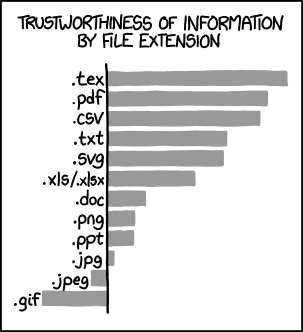
\includegraphics[width=\textwidth]{figures/file_extensions.png} 
        \caption{File Extensions} \label{fig:ext} 
    \end{subfigure}~ %add desired spacing between images, e. g. ~, \quad, \qquad, \hfill etc. %(or a blank line to force the subfigure onto a new line) 
    \begin{subfigure}[htbp]{0.5\textwidth} 
        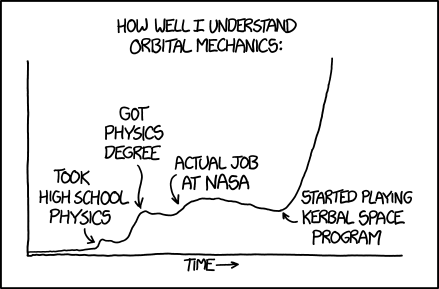
\includegraphics[width=\textwidth]{figures/orbital_mechanics.png} 
        \caption{Kerbal Space Program} \label{fig:ksp} 
    \end{subfigure}
    \caption[XKCD]{Some words of wisdom from Randall Munroe}
    \label{fig:xkcd} 
\end{figure}

\subsection{References}

Lots of famous people tend to write famous papers~\cite{newton1999}. 
Were they famous because or in-spite of their papers?
Regardless, they're famous now and we all should read them.
Certain people are so famous and do such great work that they invent a whole new field of study with a single paper~\cite{kalman1960,shannon1949}

\section{Math}

Here are some nice equations~\cref{prob_def,prob_def_constrained}
Run a manual sweep of anomalous airborne or electromagnetic readings. Radiation levels in our atmosphere have increased by 3,000 percent. Electromagnetic and subspace wave fronts approaching synchronization. What is the strength of the ship's deflector shields at maximum output? The wormhole's size and short period would make this a local phenomenon. Do you have sufficient data to compile a holographic simulation?
\begin{align}
\label{prob_def}
&\min_{s\subset W}\ J(s) = \sum_{i=1}^{l-1} H(s_j, s_{j+1}) \\
&\max_{s\subset W}\ P_{tr}(s) = \prod_{i=1}^{l-1} P_{tr}(s_j, s_{j+1}) \nonumber
\end{align}

Unidentified vessel travelling at sub warp speed, bearing 235.7. Fluctuations in energy readings from it, Captain. All transporters off. A strange set-up, but I'd say the graviton generator is depolarized. The dark colourings of the scrapes are the leavings of natural rubber, a type of non-conductive sole used by researchers experimenting with electricity. The molecules must have been partly de-phased by the anyon beam.
\begin{align}
\label{prob_def_constrained}
&\min_{s\subset W}\ J(s) = \sum_{i=1}^{l-1} H(s_j, s_{j+1}) \\
&\text{subject to} \ P_{tr}(s)>\epsilon_{tr} \nonumber
\end{align}

We're acquainted with the wormhole phenomenon, but this... Is a remarkable piece of bio-electronic engineering by which I see much of the EM spectrum ranging from heat and infrared through radio waves, et cetera, and forgive me if I've said and listened to this a thousand times. This planet's interior heat provides an abundance of geothermal energy. We need to neutralize the homing signal.



% !TEX root = ../thesis-sample.tex

\chapter{Another sample chapter}\label{chap:ipsum}

This chapter has several paragraphs of random text. 
This ensures our table of contents is correct and demonstrates how to use a multi-file \LaTeX document.

\lipsum[1]

\section{A section}
\lipsum[10]

\subsection{A subsection}
\lipsum[9]

\subsubsection{A subsubsection}
\lipsum[11]




\appendix
% !TEX root = ../thesis-sample.tex
\appendix
\chapter{Methods}
Here is how to implement the methods.

\section{Bisection}
The easiest method.

\begin{equation}\label{eq:sum}
    x_k = \frac{a_k+b_k}{2}
\end{equation}

\section{False Position}
The next one.

\chapter{Using Appendices}    \label{app:appendix}

This section might be referencing code and options that no longer exist in this version of the thesis class.
It should also be updated as well.

This appendix contains the portion of the users' manual that describes
how to use appendices with this template.  It is put in this appendix
rather than in Chapter~\cref{chap:intro} simply so that there are two
appendices, so that a list of appendices can appear earlier in the
document.

\section{Starting the Appendices}
Actually, using appendices is quite simple.  Immediately after the end
of the last chapter and before the start of the first appendix, simply
enter the command \verb|\appendix|.  This will tell \LaTeX~to change
how it interprets the commands \verb|\chapter|, \verb|\section|,
\textit{etc.}

Each appendix is actually a chapter, so once the \verb|\appendix|
command has been called, start a new appendix by simply using the
\verb|\chapter| command.

Note that the \verb|\appendix| command should be called only
once--not before the start of each appendix.



\bibliographystyle{IEEEtran}
\bibliography{thesis-bib}

% appendices must appear after
% !TEX root = ../thesis-sample.tex
\appendix
\chapter{Methods}
Here is how to implement the methods.

\section{Bisection}
The easiest method.

\begin{equation}\label{eq:sum}
    x_k = \frac{a_k+b_k}{2}
\end{equation}

\section{False Position}
The next one.

\chapter{Using Appendices}    \label{app:appendix}

This section might be referencing code and options that no longer exist in this version of the thesis class.
It should also be updated as well.

This appendix contains the portion of the users' manual that describes
how to use appendices with this template.  It is put in this appendix
rather than in Chapter~\cref{chap:intro} simply so that there are two
appendices, so that a list of appendices can appear earlier in the
document.

\section{Starting the Appendices}
Actually, using appendices is quite simple.  Immediately after the end
of the last chapter and before the start of the first appendix, simply
enter the command \verb|\appendix|.  This will tell \LaTeX~to change
how it interprets the commands \verb|\chapter|, \verb|\section|,
\textit{etc.}

Each appendix is actually a chapter, so once the \verb|\appendix|
command has been called, start a new appendix by simply using the
\verb|\chapter| command.

Note that the \verb|\appendix| command should be called only
once--not before the start of each appendix.




\end{document}
